\section{Team Evaluation}
\label{sec:04_teamEvaluation}

\change[]{correct}
Before assessing the whistle localization as whole, the three methods
to determine the sound source direction relatively
were evaluated on standalone robots in the last chapters independently.
With the results of these operations as input,
the final whistle localization outputs an absolute sound source position
with variance.
First, the start indexes were set manually to provide a decoupled result.

The size of the field used in this work is smaller than the regular \ac{SPL}
field with 7.5\si{m} length and 5\si{m} width.
Further information about the measurement setup is introduced in \cref{subsec:04_labMeasurements}.
% It is looked at the result of one exemplary measurement where the behavior
% of the team filter is of prime importance.

\subsection{Measurement Setup}
\label{subsec:04_labMeasurements}
In order to evaluate the localization methods, 11 measurement were
taken. \Cref{fig:04_setup} illustrates the positions of the Nao robots
and the positions of the whistle sound source.
According to these. the x and y values of the sources and robots are
listed in \cref{tab:04_robots} and \cref{tab:04_sources}.
The orientation $\theta$ of the robots are defined relatively to the x-axis and
corresponds to the definition in \cref{subsec:03_coordinates}.
In the following sections, the signal data from these measurements
will be used mainly.
% -------------------------------------------------------------
\btline{ht}{1.2}
\btab{|c|c|c|c|}
\hline
Nao & x [\si{m}] & y [\si{m}] & $\theta$ [\si{deg}]\\
\hline
21 & 3,75 & 2,5 & -40,2\\
\hline
24 & 3,75 & -2,5 & 90\\
\hline
26 & 0 & 0 & 0\\
\hline
27 & -3,75 & -2,5 & 66,06\\
\hline
28 & -2,45 & 0 & 0\\
\hline
\etab
\et{Positions of the robots for evaluation measurement}{04_robots}
% -------------------------------------------------------------
\btline{ht}{1.2}
\btab{|c|c|c|}
\hline
Measurement & x [\si{m}] & y [\si{m}]\\
\hline
[0] & 3,75 & 2,5\\
\hline
[1] & 3,75 & -2,5\\
\hline
[2] & -3,75 & -2,5\\
\hline
[3,9] & -3,75 & 2,5\\
\hline
[4] & -2,45 & 0\\
\hline
[5] & 2,45 & 0\\
\hline
[6,10] & 0 & 0\\
\hline
[7] & 0 & -2,5\\
\hline
[8] & -6.05 & 0\\
\hline
\etab
\et{Positions of the whistle sound sources for evaluation measurement}{04_sources}
% -------------------------------------------------------------
\begin{figure}[ht]
	\centering
		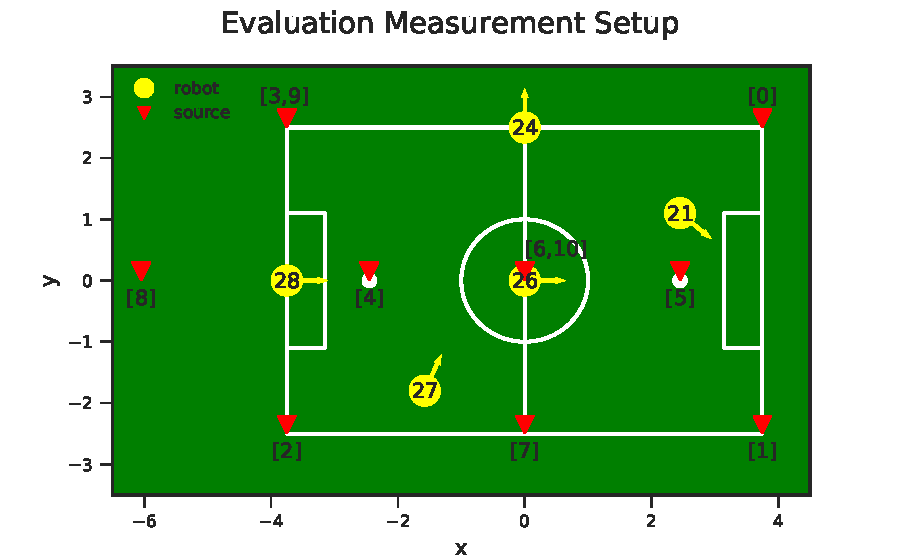
\includegraphics[]{figures/evaluation/setup}
	\caption{Setup of robots and sound source positions for the evaluation measurement.}
    \label{fig:04_setup}
\end{figure}
% -------------------------------------------------------------
\subsection{GCC Method}
\label{04_teamGcc}

To determine an overall result, each robot executes the sound source direction
detection with the \ac{GCC-PHAT} method standing alone.
After that, the results are input into the team decision filter as specified
in \cref{sec:03_teamDecision} which determines a final sound source position
result with Bayesian updating.

For further clarification, details of the result for measurement 1 of
\cref{subsec:04_labMeasurements} is presented extensively here.
\Cref{fig:04_gccResult} illustrates the result of the
relative direction angle outputs $\gamma$ of the individual robots
listed in \cref{tab:04_gccResult}.
Same as in \cref{fig:04_setup}, the yellow dots symbolizes the robots with
its orientation as short yellow line.
The resulting arrows represent the direction $\gamma$ where the sound source
is predicted.
The real source is marked as start in the graphic and the resulting
position as cross.
% -------------------------------------------------------------
\btline{ht}{1.2}
\btab{|c|c|c|c|}
\hline
Nao & $\gamma$ [\si{\deg}] & Abs. Error [\si{\deg}] & PSNR \\
\hline
21 & -26,22 & 3,71 & 18,3\\
\hline
24 & -133,77 & 9,32 & 16,8\\
\hline
26 & -30,19 & 3,50 & 19,6\\
\hline
27 & -75,26 & 1,71 & 17,4\\
\hline
28 & -15,90 & 2,53 & 15,1\\
\hline
\etab
\et{Resulting directions of the single robots with \ac{GCC-PHAT} method for a
whistle sound signal in the right front corner of the playing field}{04_gccResult}
% -------------------------------------------------------------
\begin{figure}[ht]
	\centering
		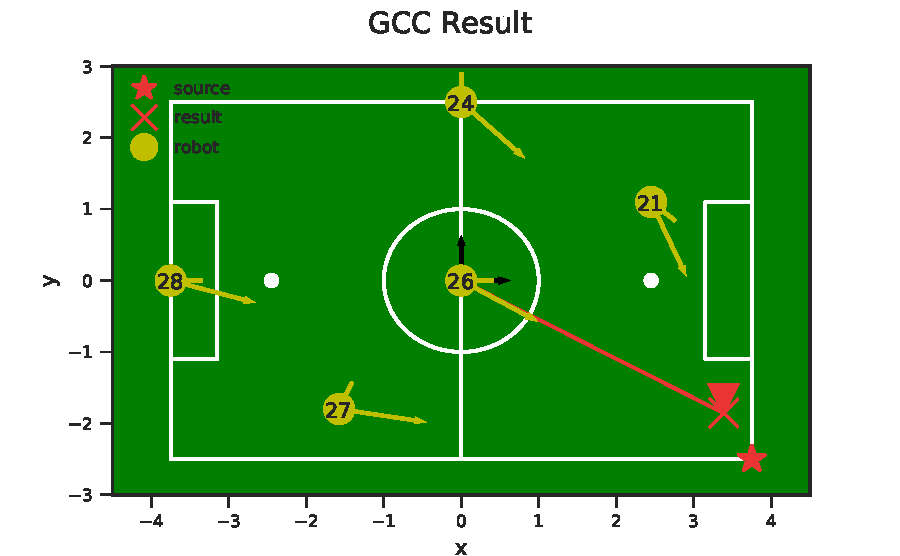
\includegraphics[]{figures/evaluation/gcc_team}
	\caption{Team whistle localization result with \ac{GCC-PHAT}
	method.}
    \label{fig:04_gccResult}
\end{figure}
% -------------------------------------------------------------

The final result and its corresponding errors are listed \cref{tab:04_gccTeamResult}.
With an absolute distance error of less than 1\si{\meter} and small angular error,
we can say that the source localization worked sufficiently.
% -------------------------------------------------------------
\btline{ht}{1.2}
\btab{|c|c|c|}
\hline
 & Result & Error\\
\hline
Position x [\si{\meter}] & 3,38 & -0,37\\
\hline
Position y [\si{\meter}] & -1,85 & 0,65\\
\hline
Angle & 33,18\si{\degree} & 1,57\si{\degree}\\
\hline
Distance [\si{\meter}] & 3,85 & 0,74 \\
\hline
\etab
\et{Whistle localization result of measurement 1 with \ac{GCC-PHAT} method}{04_gccTeamResult}
% -------------------------------------------------------------

\Cref{tab:04_gccTeamResult} shows the distance and angle errors
for all measurements in \cref{subsec:04_labMeasurements}.
The \ac{RMSE} in distance being 0.87\si{\meter} and angular \ac{RMSE}
being 5,07\si{\degree} one can say that the \ac{GCC-PHAT} algorithm
works well for whistle sound source localization.
% -------------------------------------------------------------
\btline{ht}{1.2}
\btab{|c|c|c|c|c|}
\hline
Measurement & Error x [\si{\meter}] & Error y [\si{\meter}] & Abs. Distance Error [\si{\meter}] & Angle Error\\
\hline
[0] & 1,31 & 1,06 & 1,68 & 1,45\si{\degree}\\
\hline
[1] & 0,13 & 0,06 & 0,15 & 1,57\si{\degree}\\
\hline
[2] & 0,59 & 0,43 & 0,73 & 0,42\si{\degree}\\
\hline
[3] & 0,54 & 0,47 & 0,72 & 9,09\si{\degree}\\
\hline
[4] & 0,27 & 0,0 & 0,27 & 0,01\si{\degree}\\
\hline
[5] & 0,15 & 0,14 & 0,21 & 3,18\si{\degree}\\
\hline
[6] & 0,41 & -0,02 & 0,41 & 2,67\si{\degree}\\
\hline
[7] & 0,39 & 0,02 & 0,39 & 8,98\si{\degree}\\
\hline
[8] & 1,84 & -0,01 & 1,84 & 0,14\si{\degree}\\
\hline
[9] & 0,58 & 0,52 & 0,78 & 9,89\si{\degree}\\
\hline
[10] & 0,03 & -0,0 & 0,03 & 0,0\si{\degree}\\
\hline
\etab
\et{Whistle localization results for all measurements in \cref{subsec:04_labMeasurements} with
\ac{GCC-PHAT} method}{04_gccTeamResult}
% -------------------------------------------------------------
% - intersections
% - updates
% - covariance
% - PSNR

% -------------------------------------------------------------
\subsection{CC Method}
\label{04_teamCc}

Evaluation is done of the same measurements in \cref{subsec:04_labMeasurements}
with normal \ac{CC}.
The results show that the normal \ac{CC} without weighting performs
poorer compared to the \ac{GCC-PHAT} method.
% -------------------------------------------------------------
\btline{ht}{1.2}
\btab{|c|c|c|c|c|}
\hline
Measurement & Error x [\si{\meter}] & Error y [\si{\meter}] & Abs. Distance Error [\si{\meter}] & Angle Error\\
\hline
[0] & 0,6 & 1,39 & 1,51 & 8,15\si{\degree}\\
\hline
[1] & -0,49 & 1,2 & 1,3 & 11,97\si{\degree}\\
\hline
[2] & 2,32 & 2,11 & 3,13 & 18,28\si{\degree}\\
\hline
[3] & 1,07 & -0,96 & 1,44 & 3,71\si{\degree}\\
\hline
[4] & 1,95 & -0,09 & 1,95 & 10,44\si{\degree}\\
\hline
[5] & 0,07 & 0,01 & 0,07 & 0,32\si{\degree}\\
\hline
[6] & 0,4 & -0,01 & 0,4 & 1,91\si{\degree}\\
\hline
[7] & 1,06 & -0,0 & 1,06 & 22,99\si{\degree}\\
\hline
[8] & 1,24 & -0,06 & 1,24 & 0,77\si{\degree}\\
\hline
[9] & -0,04 & 0,78 & 0,78 & 7,22\si{\degree}\\
\hline
[10] & 0,03 & -0,0 & 0,03 & 0,0\si{\degree}\\
\hline
\etab
\et{Whistle localization results for all measurements in \cref{subsec:04_labMeasurements} with
\ac{CC} method}{04_ccTeamResult}

% -------------------------------------------------------------
\subsection{Phase Method}
\label{04_teamPhase}

For the results with phase method, the minimal frequency value
parameter is set to 2700\si{\hertz}.
Just like in the previous sections, the results of the
\cref{subsec:04_labMeasurements} measurements are shown in
\cref{tab:04_phaseTeamResult} and shows the errors of the
single measurement in detail.
The \ac{RMSE} according to the distance is in the same
order of magnitude as the \ac{CC} method with 1,33\si{\meter}.
Having a much larger \ac{RMSE} regarding the angle with 74,8\si{\degree},
especially these angular errors of measurements 6 and 10 catch one's eye.
On closer examination, we see that both measurements are
taken at the center point of the field.
For the reason that the absolute position is in an acceptable
error range, we will neglect these both angular results of the
error calculation.
Thus, the angular \ac{RMSE} of the phase method without
measurements 6 and 10 is 11,69\si{\degree}.

Another conspicuous point is the number of intersections
considered in the team filter.
Compared to 
% more robots that fail -> less intersections
% show number of intersections for each file compared to method
% The rest of algorithm as presented in 03 phase
% -------------------------------------------------------------
\btline{ht}{1.2}
\btab{|c|c|c|c|c|}
\hline
Measurement & Error x [\si{\meter}] & Error y [\si{\meter}] & Abs. Distance Error [\si{\meter}] & Angle Error\\
\hline
[0] & -1,07 & -0,98 & 1,45 & 4,13\si{\degree}\\
\hline
[1] & 0,21 & 0,27 & 0,34 & 4,27\si{\degree}\\
\hline
[2] & 0,22 & 1,39 & 1,41 & 16,25\si{\degree}\\
\hline
[3] & 1,26 & -0,02 & 1,26 & 11,19\si{\degree}\\
\hline
[4] & 0,16 & -0,04 & 0,17 & 0,99\si{\degree}\\
\hline
[5] & -0,42 & 0,19 & 0,47 & 5,46\si{\degree}\\
\hline
[6] & -0,32 & 0,08 & 0,33 & 166,25\si{\degree}\\
\hline
[7] & -0,28 & 1,76 & 1,78 & 20,82\si{\degree}\\
\hline
[8] & 2,37 & 0,27 & 2,39 & 4,23\si{\degree}\\
\hline
[9] & 2,04 & 0,29 & 2,06 & 24,89\si{\degree}\\
\hline
[10] & -0,32 & 0,0 & 0,32 & 180,0\si{\degree}\\
\hline
\etab
\et{Whistle localization results for all measurements in \cref{subsec:04_labMeasurements} with
phase method}{04_phaseTeamResult}